\chapter{Introducción}

El presente documento corresponde a la realización de un Trabajo Final del Grado en Electrónica Industrial y Automática basado en la conexión e integración de un brazo robótico en una red domótica. A continuación, se recoge de manera ordenada y detallada el desarrollo e implementación del proyecto; así como los resultados obtenidos y las conclusiones a kas que es posible llegar.

\section{Motivación del proyecto}

El punto de partida es el proyecto Robohealth. Consiste en un conjunto de entidades en colaboración para el desarrollo de soluciones relacionadas con la robótica y la domótica con el fin de introducir mejoras en el sistema sanitario. Como se puede observar, entre estas entidades está, además de otras dos universidades públicas de la Comunidad de Madrid, la Universidad Politécnica de Madrid.

Los resultados del proyecto están orientados a pacientes con enfermedades crónicas o capacidades cognitivas limitadas, pacientes en una situación de dependencia a los que es posible mejorar la calidad de vida. Estas mejoras se obtienen a través del diseño y fabricación de robots de asistencia, tanto para pacientes como para sus cuidadores, y la implementación de entornos inteligentes.

En la figura \ref{fig:RH}, se pueden observar los diferentes paquetes de trabajo y subproyectos en los que se trabaja dentro de la estructura de RoboHealth, repartidos entre las entidades colaboradoras. En la Universidad Politécnica de Madrid, encargada del desarrollo de entornos inteligentes de asistencia y rehabilitación, se ha venido trabajando en distintas herramientas enmarcadas en Trabajos Finales de Grado durante los últimos años.

\begin{figure}[tb]
\centering
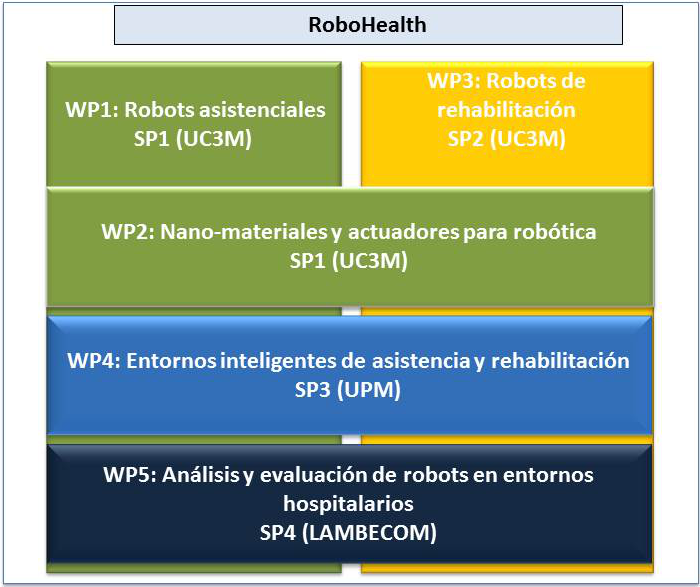
\includegraphics[width=0.55\textwidth]{figuras/RHstruct.png}
\caption{Estructura RoboHealth}
\label{fig:RH}
\end{figure}

Dentro del marco previamente expuesto, se han desarrollado dos plataformas que sirven de base para el proyecto objetivo de este documento.

\begin{itemize}
\item \textbf{RoboHealth Arm} es un brazo robótico de tres grados de libertad (actualmente, cuenta con sólo dos grados de libertad operativos) diseñado para sustentar una tablet en su extremo, haciendo más acesible su uso para pacientes y cuidadores. Está basado en un sitema de cuerdas y poleas accionado por tres servomotores.
\item Por otro lado, existe una aplicacion de \textbf{Node-RED} que integra los diferentes dispositivos y proyectos desarrollados en una red domótica. Incluye una interfaz gráfica que facilita su interacción vía internet, posibilitando controlar los dispositivos desde cualquier lugar.
\end{itemize} 

La idea es continuar el proceso de integración de los diferentes dispositivos en Node-RED con la intención de controlar todo desde la misma interfaz. En ese contexto, surge el proyecto de hacerlo con el brazo RoboHealth Arm. Con el fin de tratar de explorar todas las tecnologías posibles, se comprueba que la radiofrecuencia aún no habia sido y existen soluciones económicas en el mercado.

Así, el planteamient del Trabajo Final de Grado tomó forma, defiendose como la conexión mediante el uso de radiofrecuencia del brazo RoboHealth Arm a la interfaz de Node-RED. Para la radiofrecuencia, se usarán dispositivos XBee.

\section{Objetivos}

El fin del proyecto es la completa integración de un control a través de internet del brazo robótico. Los comandos se lanzan desde la interfaz de Node-Red y el ordenador de la sala transmite la orden vía radiofrecuencia al brazo.

Se ha desarrollado a posibilidad de configurar las coordenadas articulares del brazo antes de ser enviadas, dentro de su rango óptimo de trabajo actual.

La orden de Node-Red pone en marcha la ejecución de un script en Python que toma esos parámetros previamente especificados y envía por uno de los puertos serie el correspondiente frame. Este frame está pensado de acuerdo a las especificaciones de comunicación del brazo y del encapsulamiento de las comunicaciones de radio.

Un dispositivo XBee ha sido configurado para enviar el frame de datos recibido por comunicación serial. Al poder concentrarse todo el procesamiento de la información correspondiente al emisor en el anteriormente mencionado script, no se precisa de ningún microcontrolador adicional que funcione junto al módulo de radiofrecuencia. Así pues, el módulo XBee funciona de manera exclusiva como un traductor entre la información en el puerto serie correspondiente y las ondas de radiofrecuencia.

El dispositivo XBee receptor de la información que comanda el brazo robótico esta situado en el mismo. Su objetivo es ser capaz de captar el mensaje de radio específicamente diseñado para él y transmitirlo al microcontrolador del brazo. De la misma manera que en el otro XBee, su función será la de traductor de las ondas de radio (excusivamente de las destinadas a él) en información en el puerto serial. Esto es posible gracias al prediseño de los frames de información de acuerdo a las especificaciones y protocolos de comunicación del brazo.

El dispositivo operativo provoca la reacción esperada en el brazo, moviendo sus servos hasta las coordenadas articulares especificadas.

\section{Materiales utilizados}

Aquí se pueden citar todos los materiales utilizados, tanto software como hardware, para que el lector tenga una primera de lo que se va a hablar en el TFG.

\subsection{Componentes hardware}

\subsection{Componentes software}

\section{Estructura del documento}

A continuación y para facilitar la lectura del documento, se detalla el contenido de cada capítulo.

\begin{itemize}
\item En el capítulo 1 se realiza una introducción.
\item En el capítulo 2 se hace un repaso...
\end{itemize}
